\chapter{L'identificazione della curva}
L'algoritmo di identificazione della curva è composto da diverse funzioni, ciascuna di esse svolge delle operazioni sui dati ottenuti dall'algoritmo del pathShape, che permettono di estrarre i dati necessari per eseguire il confronto tra una eventuale curva identificata nell'immagine (catturata dalla telecamera frontale) e la lista delle curve presenti nel percorso.

Una prima funzione si occupa di riordinare e normalizzare i dati. Si procede quindi a segnare i dati punto per punto, utilizzando come criterio il comportamento di ogni dato rispetto a quello successivo. Per finire si utilizzano i dati estratti sul comportamento per calcolare i parametri delle curve visibili nell'immagine, che verranno infine usati per il confronto.

\section{L'aggiustamento dei dati dell'algoritmo di pathshape}

    Come analizzato nel precedente capitolo l'algoritmo di pathshape ritornare una matrice di vettori 3$\times$N, nella quale ciascun vettore contiene le coordinate $(x, y, \alpha)$ di un punto all'interno della curva. $\alpha$ è equivalente all'angolo di curvatura della linea nel punto considerato dal pathShape.

Le prime due problematiche affrontate sono state:
\begin{itemize}
    \item I punti ritornati dal pathshape non erano ordinati, quindi è stato necessario riordinarli prima di svolgere qualsiasi altra operazione. \'E infatti necessario che i dati siano in ordine per svolgere le operazioni successive con più efficenza.
    \item Tra i punti ritornati dal pathshape si riscontravano delle leggere fluttuazioni e si avevano spesso situazioni in cui un punto era leggermente spostato verso un lato della linea, mentre il successivo risultava leggermente spostato verso il lato opposto. Questa problematica è stata riscontrata soprattutto nel caso di punti all'interno di una linea curva. Si è reso quindi necessario l'uso di una funzione che regolarizzasse leggermente i dati.
\end{itemize}

Il primo problema è stato risolto modificando l'algoritmo del pathshape. L'algoritmo infatti, dopo una fase di ricerca nella parte dell'immagine soprastante il primo punto identificato, cominciava una fase di ricerca nella parte sottostante. Questo portava ad avere una matrice in cui gli ultimi k vettori risultavano essere le posizioni più vicine al punto mantenuto a fianco del robot seguendo la linea. Sapendo questo è bastato modificare l'algoritmo in modo da salvarsi un valore che indicasse l'indice in cui questa inversione avveniva, in modo da riordinare subito dopo la matrice. \'E possibile infatti spostare i vettori apparsi dopo l'indice salvato all'inizio della matrice, spostando in avanti il resto dei dati con complessità O(n). Il raggiungimento dell'obiettivo con complessità lineare è importante per ridurre il tempo di calcolo necessario.

Per risolvere la seconda problematica è stato deciso di adottare un algoritmo che calcoli una media pesata dei punti intorno al punto considerato. Questo metodo consiste nel sostituire ogni punto $p_i = (x_i, y_i, \alpha_i)$ con il nuovo punto ottenuto $\overline{p_i} = (\overline{x_i}, \overline{y_i}, \overline{\alpha_i})$, riducendo significativamente le fluttuazioni all'interno della matrice. La funzione lavora quindi su ogni punto singolarmente facendo una media pesata del punto considerato con i 4 elementi più vicini. Ai valori più distanti viene assegnato un peso minore, in modo da influnenzare il risultato in maniera minore e ottenere una matrice di punti con un andamento più dolce, senza che questi siano eccessivamente influenzati dai punti intorno.
Quindi il nuovo punto $\overline{p_i}$ viene calcolato come $$\overline{p_i} = {w_1\cdot (p_{i-2}+p_{i+2})+w_2\cdot (p_{i-1}+p_{i+1})+p_i \over 2\cdot w_1+2\cdot w_2+1}$$
con $w_1$ e $w_2$ come pesi assegnati e $w_1 < w_2$.
\begin{figure}[!ht]
    \centering
    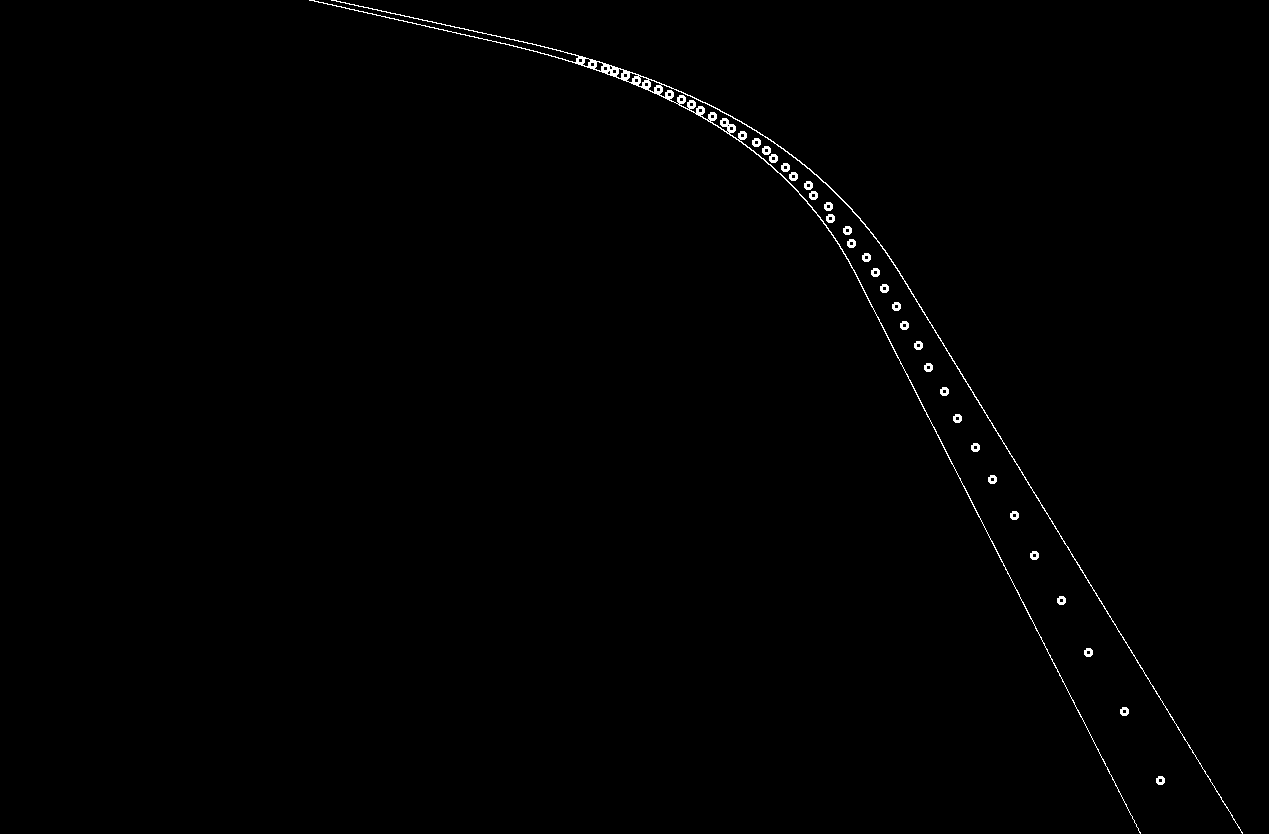
\includegraphics[width=0.8\textwidth]{img/pathshapeoriginal}
    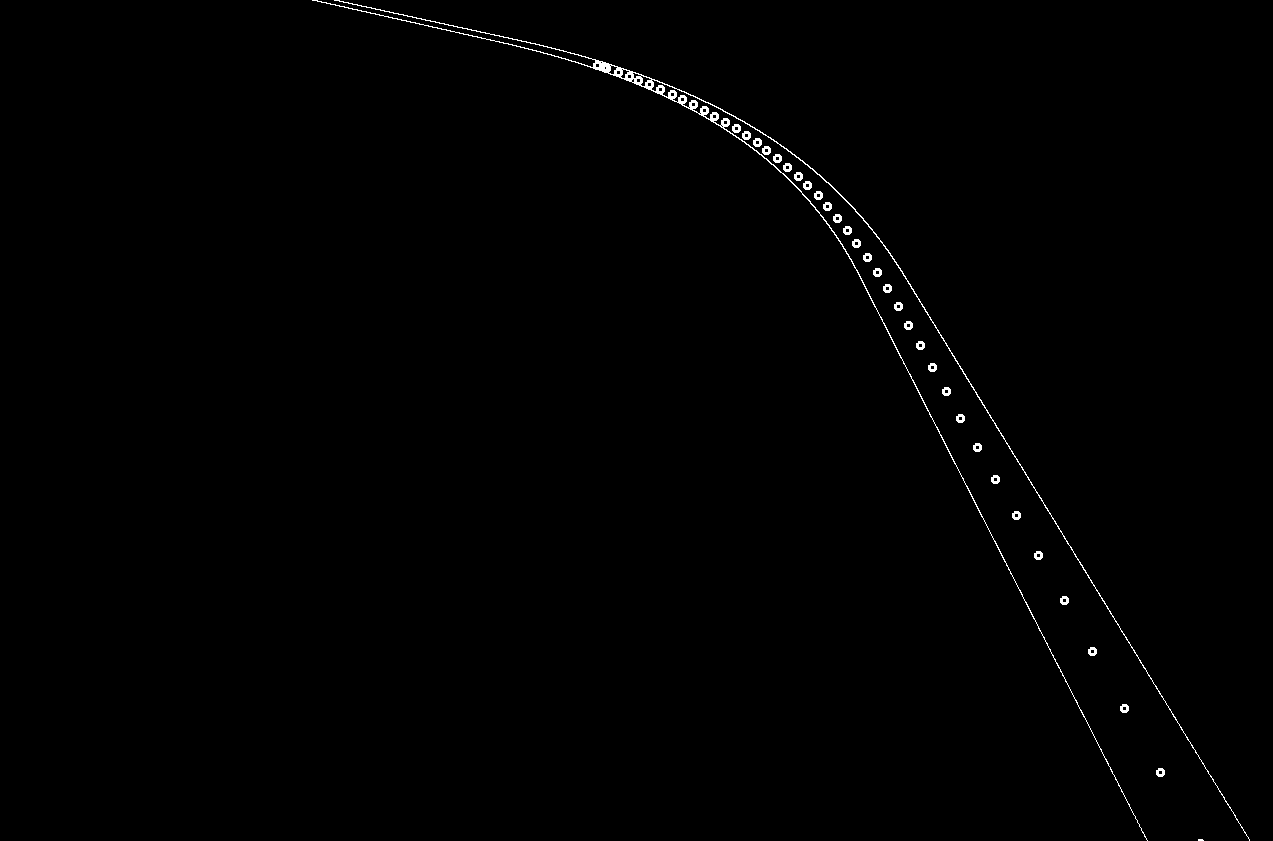
\includegraphics[width=0.8\textwidth]{img/pathshapefilter}
    \caption[Punti restituiti dall'algoritmo pathshape prima del filtro.]{Esempio di come risultavano i punti restituiti dall'algoritmo del pathshape prima (sopra) e dopo (sotto) aver applicato la funzione per regolarizzarne i dati.}
\end{figure}

\section{Lo studio dell'angolazione nei singoli punti della curva}

    Risolti i problemi riguardanti i dati del pathshape si rende necessario identificare quando il percorso sta curvando e quando sta procedendo in linea retta. È quindi necessario avere una misura della variazione dell'angolo  tra un punto e il successivo. Inizialmente è stato necessario ricavare un vettore contenente tutte le differenze  tra un punto e il successivo $\delta_{i} = \alpha_i-\alpha_{i+1}$. Da questo è stato sviluppato un semplice algoritmo che scorrendo i punti marca ciascuno di essi con un numero che indica il suo comportamento, ovvero lo spostamento verso destra, lo spostamento verso sinistra o lo spostamento in linea retta.

    Questo risultato è stato ottenuto attraverso un algoritmo che linearmente scorre il vettore delle differenze e per ogni punto effettua un controllo sul valore della differenza, sapendo che nel caso di spostamenti a destra $\delta_i$ mantiene un valore a segno positivo, viceversa a valori di $\delta_i$ positivi si assoceranno piccoli spostamenti verso sinistra. Si procede quindi a marcare il punto utilizzando un sistema di regole rigide basate su dei valori fissi \(W_1\) e \(W_2\), con \(W_1>W_2\) (da non confondere con i pesi $w_1$ e $w_2$ usati precedentemente). Questi due valori sono sono impostati al valore di \(W_1 \mapsto 0.065 \cdot pshapeStep\) e \(W_2 \mapsto 0.015 \cdot pshapeStep \), sono quindi dipendenti dalla lunghezza del passo impostato nell'algoritmo di pathshape. Questo perchè il valore di $\delta$ dipende direttamente dalla larghezza del passo compiuto quindi senza questo accorgimento sarebbe necessario normalizzare i valori di $\delta$ per il valore di $pshapeStep$.

    L'algoritmo mantiene in memoria l'ultimo valore assegnato: $flag_{prec}$, e utilizza un contatore in modo da garantire una leggera resistenza nel passaggio da un caso in cui i punti siano posti in curva al caso in cui in punti successivi siano parte di un rettilineo. Questo accorgimento è stato adottato per evitare che degli errori nell'algoritmo di pathShape possano alterare il risultato. Andiamo quindi ad analizzare le regole con cui vengono marcati i singoli punti:

    \begin{itemize}
        \item Se il punto risulta angolato di un valore $\delta_i$ con $\delta_i > W_1$ o $\delta_i < -W_1$, viene immediatamente marcato come un punto in curva, a sinistra nel primo caso: $flag_i \mapsto -1$ o a destra nel secondo caso: $flag_i \mapsto 1$.
        \item Se il punto risulta angolato di un valore $\delta_i$, con $W_1>\delta_i>W_2$ o $-W_2>\delta_i>-W_1$, si mantiene il valore del flag precedentemente usato, a meno che $\delta_i$ non indichi uno spostamento inverso rispetto a quello indicato da $flag_{prec}$: caso in cui $flag_{prec} = -1 \land \delta_i<0$, caso in cui $flag_{prec} = 1 \land \delta_i>0$. In questi casi si ritorna in una situazione di rettilineo $flag_i \mapsto 0$.
        \item Se il valore soddisfa invece il seguente criterio: $W_2>\delta_i>-W_2$, allora l'algoritmo controlla il valore dal contatore $c$. Se $c>2$, quindi se ci sono stati almeno altri 2 punti entro il range di valori considerato prima di quello corrente, allora imposta il valore del punto corrente marcandolo come parte di un rettilineo, altrimenti incrementa di 1 il contatore c.
        Questo meccanismo di fatto sospende l'assegnazione di un valore di $flag_i$ per alcuni punti, il che rende necessario controllare il valore di $c$ ogni volta che si assegna un valore a $flag_i$ ed eventualmente assegnare lo stesso valore anche ai $k$ punti lasciati in sospeso.
    \end{itemize}
    \begin{figure}[!ht]
        \centering
        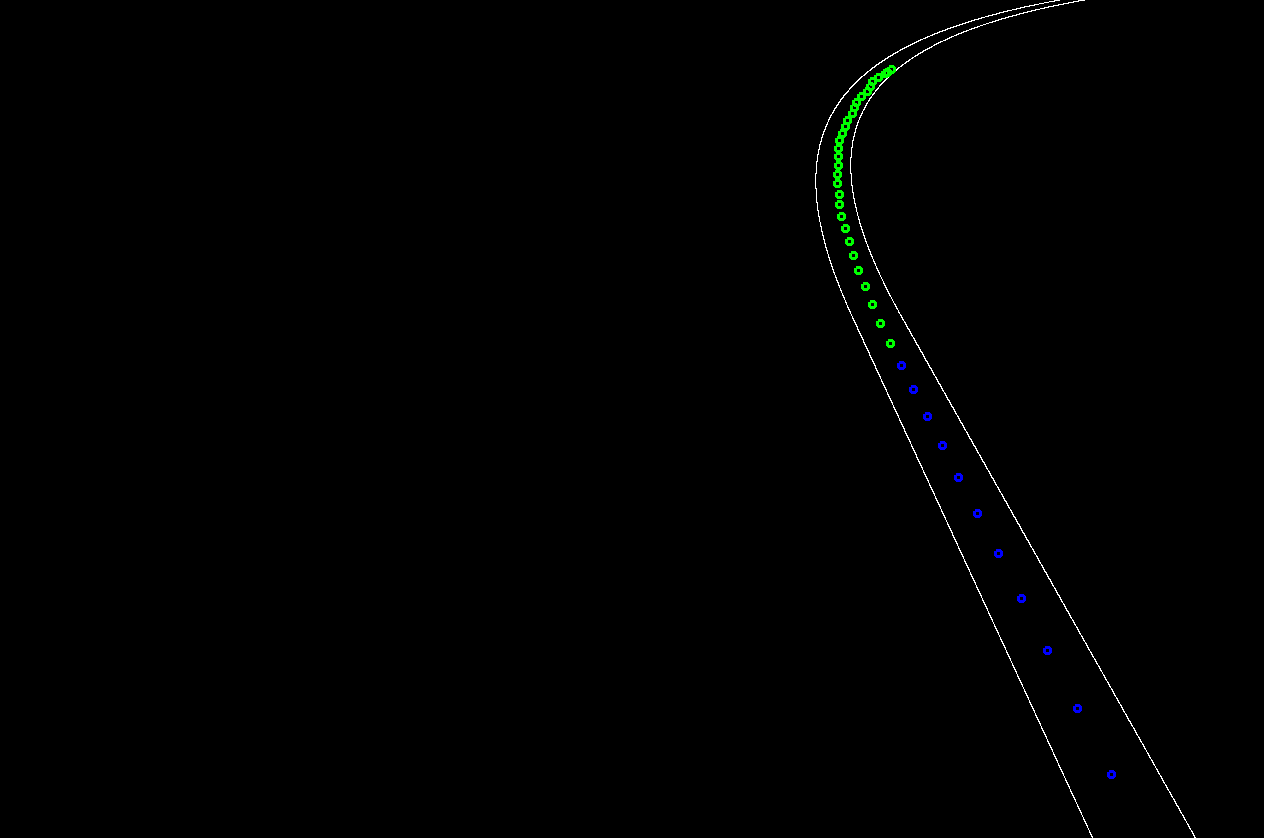
\includegraphics[width=0.75\textwidth]{img/pathcurve1}
        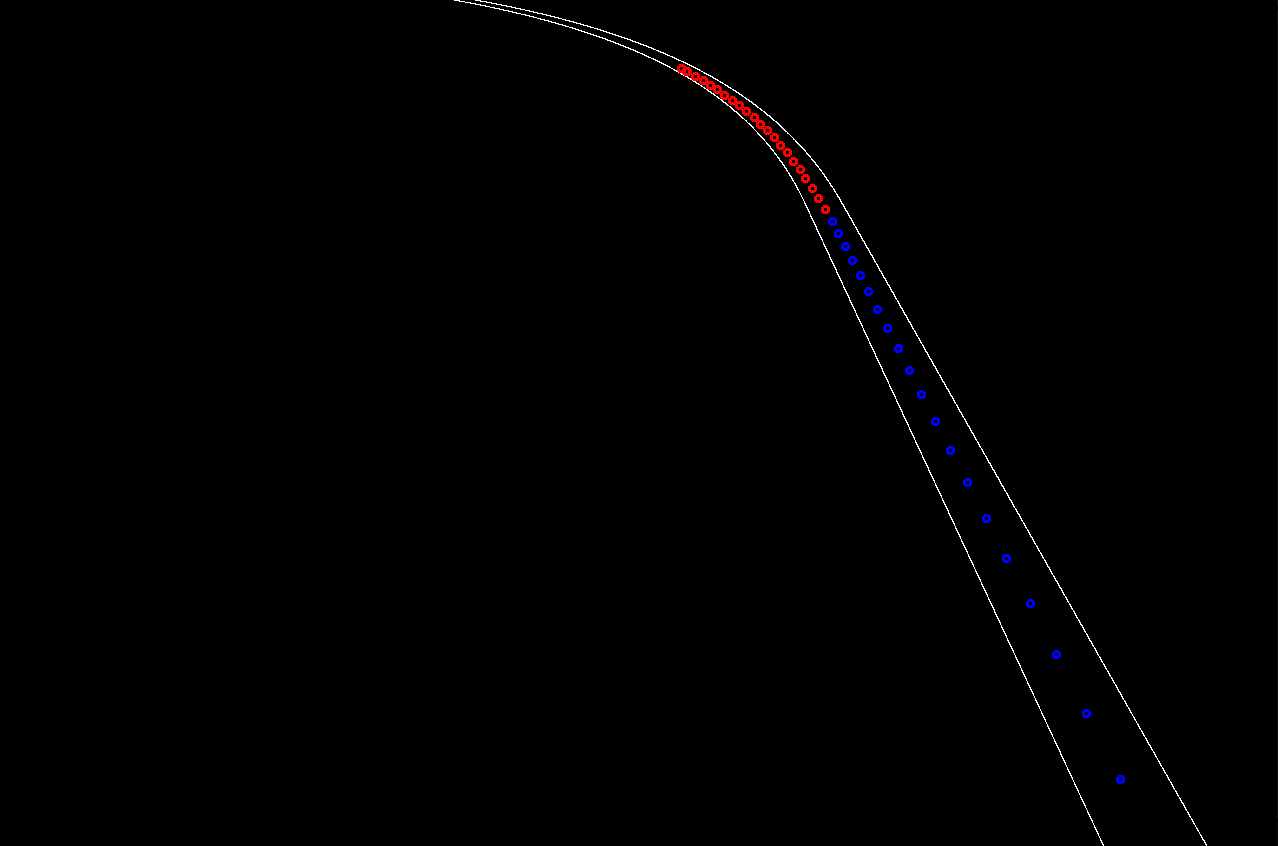
\includegraphics[width=0.75\textwidth]{img/pathcurve2}
        \caption[Risultati dell'algoritmo di studio della curva.]{In queste due immagini possiamo osservare un paio di risultati dell'algoritmo di studio della curva: blu nel caso il punto sia in rettilineo, rosso se viene identificata una curvatura verso sinistra, verde se invece il percorso sta curvando verso destra}
    \end{figure}

\section{La procedura di calcolo dei parametri della curva}

    Una volta che ciascuno dei punti è stato marcato il risultato viene passato alla funzione \textit{findCurvature}. La funzione in una prima fase separa le curve identificate nell'immagine, quindi per ognuna di esse svolge una serie di calcoli necessari a trovare i parametri necessari. In primo luogo applica una decomposizione a valori singolari tra una prima matrice N$\times$3, con N numero di punti nella curva e costruita nel seguente modo:\newline
    $$\begin{bmatrix}x_0 & y_0 & 1 \\ x_1 & y_1 & 1 \\ \vdots & \vdots & \vdots \\ x_n & y_n & 1 \end{bmatrix}$$ e un secondo vettore di dimensione N costruito nel seguente modo: \newline
    $$\begin{bmatrix}-(x_0^2+y_0^2) \\ -(x_1^2+y_1^2) \\ \vdots \\ -(x_n^2+y_n^2) \end{bmatrix}$$
    dal risultante vettore $X$ di dimensione 3 è possibile ottenere il raggio e il centro dell'arco di curvatura nel modo seguente: \newline
    $$ r = \sqrt{{\tfrac{X_0^2+X_1^2}{4}}-X_2}$$
    $$ x_c = \tfrac{X_0}{2} $$
    $$ y_c = \tfrac{X_1}{2} $$

    Ottenuti raggio e centro dell'arco di curva possiamo calcolare l'angolo dell'arco trovato usando le coordinate del punto iniziale dell'arco $I = (x_i, y_i)$, le coordinate dell'ultimo punto dell'arco $F = (x_f, y_f)$ e le coordinate del centro dell'arco di curva $C = (x_c, y_c)$. Come primo passo è quindi necessario identificare la distanza tra il punto finale dell'arco di curva e il segmento costituito dal centro dell'arco appena calcolato e il punto iniziale dell'arco di curva nel seguente modo:

    \begin{figure}[!ht]
        \centering
        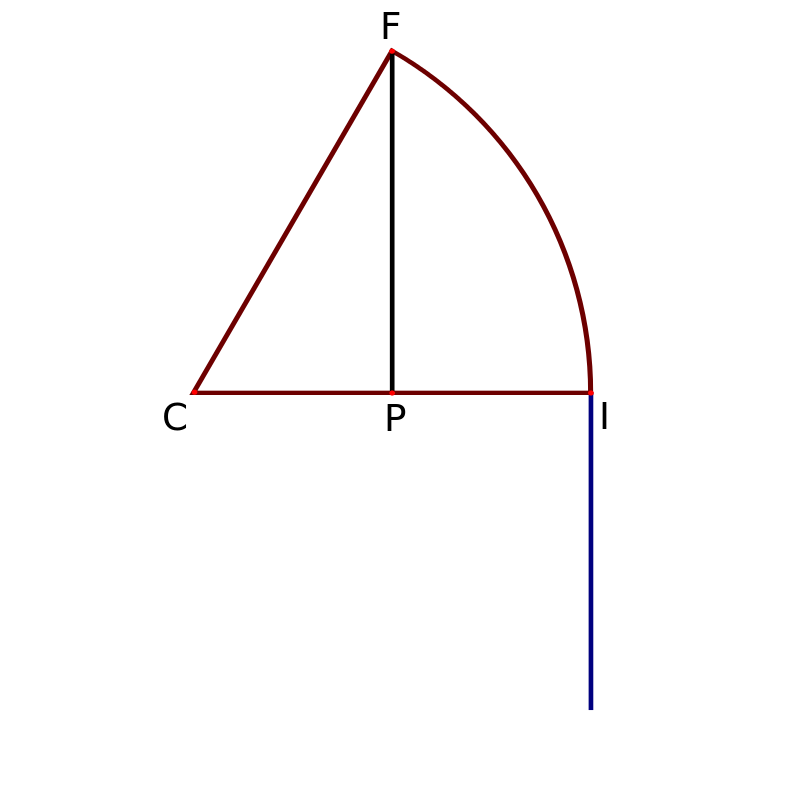
\includegraphics[width=0.6\textwidth]{img/curveimg}
        \caption[Immagine della curva.]{Rappresentazione visuale degli elementi utilizzati in questa sezione.}
    \end{figure}

    $$l = (x_i-x_c)^2+(y_i-y_c)^2$$
    $$u = {(x_f-x_i) \cdot (x_c-x_i) + (y_f-y_i) \cdot (y_c-y_i) \over l} $$
    A questo punto è possibile trovare le coordinate del punto $P$ di intersezione tra il segmento $\overline{I C}$ e la sua perpendicolare passante per $F$ (riferimento alla figura 3.3):
    $$(x_p, y_p) = (x_i+u*(x_c-x_i), y_i+u*(y_c-y_i))$$
    Da qui si può calcolare da distanza $\overline{F P}$ e risolvere l'angolo $\theta$ utilizzando l'arcoseno:
    $$d = \sqrt{(x_p-x_f)^2+(y_p-y_f)^2}$$
    $$\theta = \arcsin^{-1}(d/r)$$
    Una volta compiute le operazioni sopra descritte viene restituita una matrice contenente i parametri delle $k$ curve che appaiono nell'immagine, costruita nel modo seguente:
    $$\begin{bmatrix} flag_1 & \theta_1 & x_{c_1} & y_{c_1} & r_1 \\ \vdots & \vdots & \vdots & \vdots & \vdots \\ flag_n & \theta_n & x_{c_n} & y_{c_n} & r_n \end{bmatrix}$$
    Tutte le curve che hanno meno di 5 punti identificati dall'algoritmo di pathshape vengono scartate, in quanto nonostante il processo di aggiustamento dei punti le piccole fluttuazione di essi possono completamente fuorviare i risultati.

\section{Il processo di confronto}

    Il confronto tra curve deve risolvere un problema fondamentale, è infatti necessario avere una misura di distanza tra le curve in modo da poter identificare curve simili. In questo caso è possibile risolvere il problema usando una funzione che calcola la differenza tra i parametri di due curve date, ritornando un valore numerico ottenuto sommando le differenze dei parametri in input alla funzione.
    I parametri considerati dalla funzione di distanza sono
    \begin{itemize}
        \item \textbf{Il flag assegnato alle curve:} è il parametro considerato come il più importante, infatti una differenza su questo valore indica che le due curve confrontate si sviluppano in direzioni diverse quindi è impossibile che le due curve siano simili. La funzione di distanza è quindi programmata per restituire un numero grande in questo caso.
        \item \textbf{Il raggio della curva:} la funzione processa questo parametro con una semplice differenza in valore assoluto $\delta_r = |r_1-r_2|$ sommata poi al valore restituito.
        \item \textbf{L'angolo di curvatura:} questo caso risulta leggermente più complicato dei precedenti, infatti la scarsa distanza a cui l'algoritmo di pathshape identifica la linea sul terreno rende complicato ottenere un angolo di curvatura corretto.
        \'E quindi necessario distinguere tra il caso in cui l'angolo di curvatura calcolato risulti minore dell'angolo da confrontare $\alpha_1<\alpha_2$ e il caso inverso $\alpha_1>\alpha_2$, assegnando dei pesi diversi ai due casi. Nel primo caso possiamo assumere che la curva non sia stata identificata completamente quindi assegneremo un peso basso alla differenza. $$\delta_{\alpha} = |\alpha_1-\alpha_2|*0.1$$    Nel secondo caso invece, nonostante la curva non sia stata completamente identificata, possiamo osservare una parte di curva maggiore rispetto alla curva usata come confronto, quindi non assegnamo nessun peso alla differenza in questo caso $\delta_{\alpha} = |\alpha_1-\alpha_2|$
    \end{itemize}
    Il valore di ritorno della funzione di distanza viene quindi calcolato come: $$ret = \delta_r+\delta_{\alpha}$$
    Risolto il problema della funzione di distanza la parte di confronto risulta un semplice calcolo del minimo tra le distanze. La curva identificata nell'immagine viene confrontata con una serie di curve date in input dal programmatore (che può quindi gestirsi la posizione ottenuta dagli encoder per inserire solo i parametri delle curve presumibilmente vicine al robot). Se i valori di distanza di una o più curve risultano abbastanza vicini vengono ritornati i valori di distanza calcolati e gli indici corrispondenti nella matrice data in input dal programmatore. In caso contrario viene restituita una matrice vuota.
